\documentclass{ximera}
\usepackage[colorlinks=true,urlcolor=blue]{hyperref}
\title{Setting up the repository}
\begin{document}
\begin{abstract}
Instructions for setting up a repository containing course materials.
\end{abstract}
\maketitle

This tutorial is intended to help course instructors get a
\href{http://ximera.osu.edu}{\sf Ximera} 
course up and running. It guides the reader through the creation of 
a git repository, the connection of the repository to
\href{http://github.com}{\tt github.com}
through a webhook, and the creation of an activity containing some 
simple exercises.

The instructions below assume that the reader will be
working on a computer running either Linux or OS X.
Similar instructions for Windows users will be composed
at a later stage, but the Linux instructions below will probably
be sufficient for Windows users with some familiarity with Unix commands.
While the reader could in principle avoid installing 
\href{http://texlive.org}{\LaTeX}\
and \href{http://git-scm.com}{\sf git} these programs are necessary
to take full advantage of the features of the 
\href{http://ximera.osu.edu}{\sf Ximera} system.

\begin{enumerate}
\item Create a directory for your course files
and change to that directory.
In this example, we will create a directory called
\verb!anExampleCourse!.
Open a terminal session and type the following commands.
\begin{center}
\begin{verbatim}
mkdir anExampleCourse
cd anExampleCourse 
\end{verbatim}
\end{center}

\item A Ximera course consists of a directory (the one
created above in this example)
containing a text file called \verb!course.xim!. 
In this tutorial we will create a simple
course that has only one activity.
Using any text editor,
create and save a file named
\verb!course.xim! containing the content below.

\begin{verbatim}
---
name: An example course
description: This is a Ximera activity explaining how to get started with Ximera for course instructors.
---

theFirstActivity/theFirstActivity
\end{verbatim}
\begin{warning}
The content of the line beginning with \verb!name:!
specifies the title of your course exactly as it will appear on
\href{http://ximera.osu.edu/course}{\tt ximera.osu.edu/course}.
So in this example, the course will appear
as \verb!An example course!.
In order to distinguish your course from
other courses on
\href{http://ximera.osu.edu/course}{\tt ximera.osu.edu/course}
you should change the title to something unique
such as \verb!ISU Math 104!.
\end{warning}

\begin{remark}
In general the file \verb!course.xim! specifies course information
such as the name of the course, a description of the course,
and the names of all \LaTeX\ activity files 
comprising the course, in the order
they should be presented to students.
In addition to a name and description,
the \verb!course.xim! file above specifies that 
there is one activity file \verb!theFirstActivity.tex!,
written without the extension \verb!.tex!,  
located in a directory called \verb!theFirstActivity!.
We will create this file and directory in the following step.

Generally courses should contain more than one activity,
with each activity filename appearing in \verb!course.xim!
without the \verb!.tex! extension and
indented to reflect its position in the course hierarchy.
We recommend placing each
activity in its own directory, which should have the same name.
This facilitates
sharing activities among collaborators and makes reusing existing
activities easier.
%Later in this course, we will see examples of
%how to borrow existing activities from other courses
%rather than starting from scratch. 
We also recommend that the \LaTeX\ file have exactly
the same name as the title of the activity,
with all spaces removed and all words other than the first
capitalized. So for example, if the title of the
activity were \verb!Plants native to Ohio!
the \LaTeX\ file \verb!plantsNativeToOhio.tex!
would be located in a directory called
\verb!plantsNativeToOhio!.
\end{remark}

\begin{warning}
The \verb!course.xim! file has particular formatting requirements.
\begin{enumerate}
\item The name of the file must be exactly \verb!course.xim!
\item The \verb!---!'s encapsulating the name on line~2
and the description on line~3
are required, as is the blank line following the second \verb!---!.
\item Both entries between the \verb!---!'s must exist as single lines. 
In other words, the only newlines permitted are those
at the end of lines~2 and 3.
\end{enumerate}
\end{warning}

\item In your terminal create a new directory
in the \verb!anExampleCourse! directory
called \verb!theFirstActivity!. The \verb!theFirstActivity!
directory should contain a file called \verb!theFirstActivity.tex!.
This can be accomplished by
executing the commands below.
\begin{verbatim}
mkdir theFirstActivity 
cd theFirstActivity 
touch theFirstActivity.tex
\end{verbatim}

\item Using your text editor, open \verb!theFirstActivity.tex!
and paste the following content. Then save the file.
\begin{verbatim}
\documentclass{ximera}
\title{The First Activity}
\begin{document}
\begin{abstract}
This activity deals with \verb!Ximera! activities
\end{abstract}
\maketitle
\end{document}
\end{verbatim}

\begin{remark}
An activity should be in the document class \verb!ximera!
and should contain the title of the activity
and an abstract. At this stage the activity above has
a title and abstract, but is otherwise blank.
\end{remark}

\item Log into your \href{http://github.com}{\tt github.com}
account and
create a repository with the same name as your top directory
\verb!anExampleCourse!
by clicking the \verb!+! by your account name, as shown
below.

\begin{image}
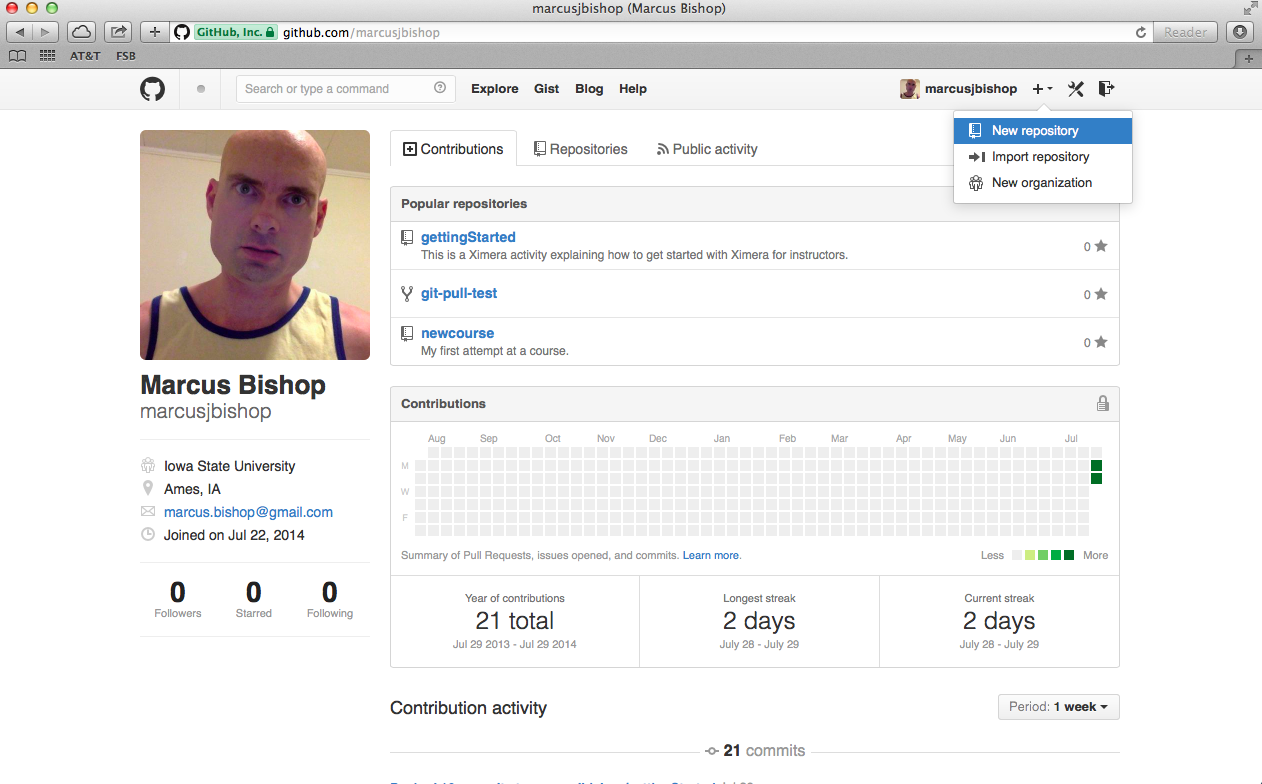
\includegraphics[scale=.3]{RepoInit.png}
\end{image}

After selecting \verb!New repository!, a new
page appears with a field named \verb!Repository name!. Enter
\verb!anExampleCourse! into this field and
accept all default settings by pressing the
\verb!Create Repository! button.
\begin{image}
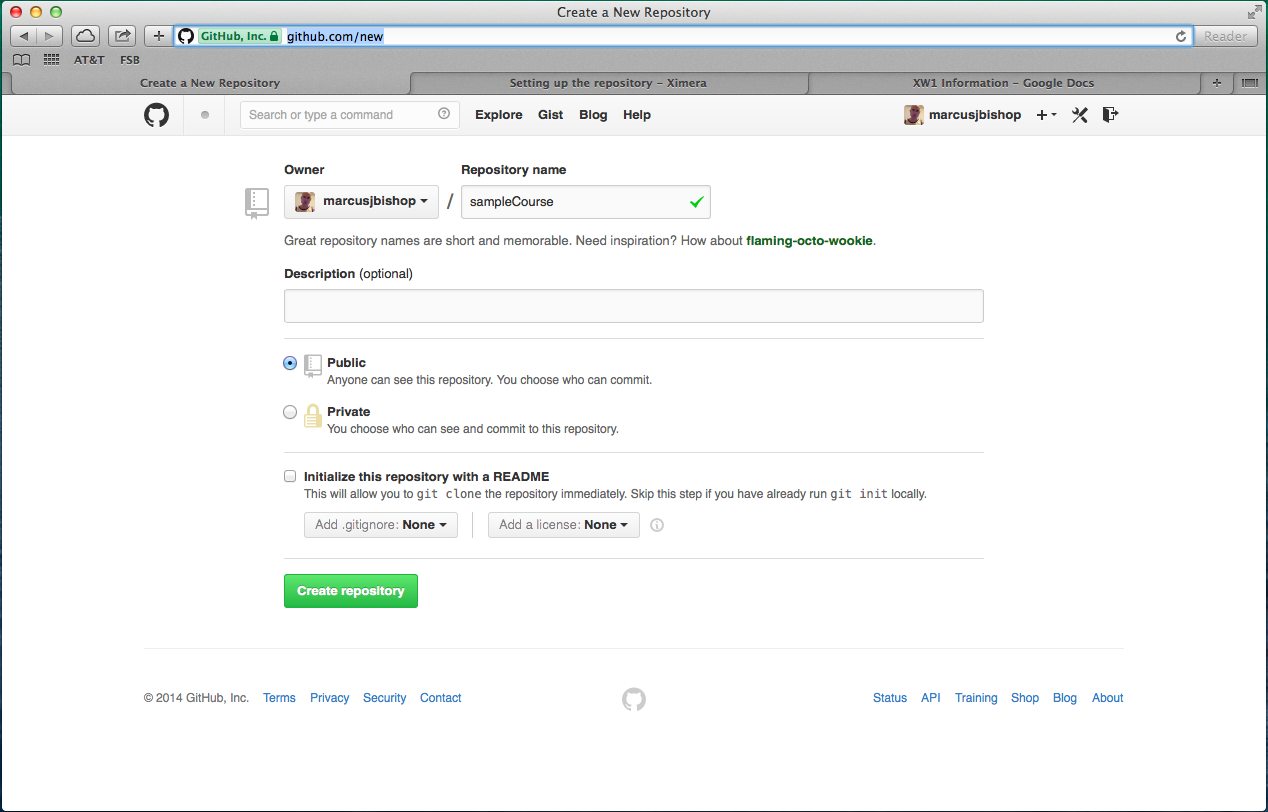
\includegraphics[scale=.3]{CreateRepo.png}
\end{image}
\href{http://github.com}{\tt github.com}
will respond with additional commands similar to
those shown below.
\begin{verbatim}
touch README.md
git init
git add README.md
git commit -m "first commit"
git remote add origin https://github.com/marcusjbishop/anExampleCourse.git
git push -u origin master
\end{verbatim}
Before executing these commands, return
to your terminal and ensure that your current directory is
the root directory \verb!anExampleCourse! of your repository.
If your current directory is \verb!theFirstActivity!
from the previous step you can change to the parent directory by typing
\begin{verbatim}
cd ..
\end{verbatim}
Now execute the commands returned by
\href{http://github.com}{\tt github.com}.

\begin{remark}
Note that your username appears in the fifth line
of these commands in place of \verb!marcusjbishop!.
Note also the \verb!s! in \verb!https!.
These commands initialize the repository on \href{http://github.com}{\tt github.com}
and create an empty file named \verb!README.md!
in the \verb!anExampleCourse! directory.
\end{remark}

\item Execute the following command.
\begin{verbatim}
git add .
\end{verbatim}
\begin{remark}
Note that the command contains a dot.
The command adds the newly created directory
\verb!theFirstActivity! and the files
\verb!theFirstActivity/theFirstActivity.tex!
and \verb!course.xim! to the your repository.
In general the command above must be executed
every time a new file or directory is created.
\end{remark}

\item This step is optional. Add a
description of your course to the file
\verb!README.md!.

\begin{remark}
In general the content of \verb!README.md! should
provide a description of your project that will appear only on
\href{http://github.com}{\tt github.com}.
\end{remark}

\item Click on the \verb!Settings! button on the
\href{http://github.com}{\tt github.com} repository page
and then on \verb!Webhooks & Services!.
Now click the \verb!Add webhook! button.
Type \verb!http://ximera.osu.edu/github!
into the \verb!Payload URL! field and
\verb!8mi0tsrje9n3asPu86XC198G1XSdZj!
into the \verb!Secret! field.
\begin{image}
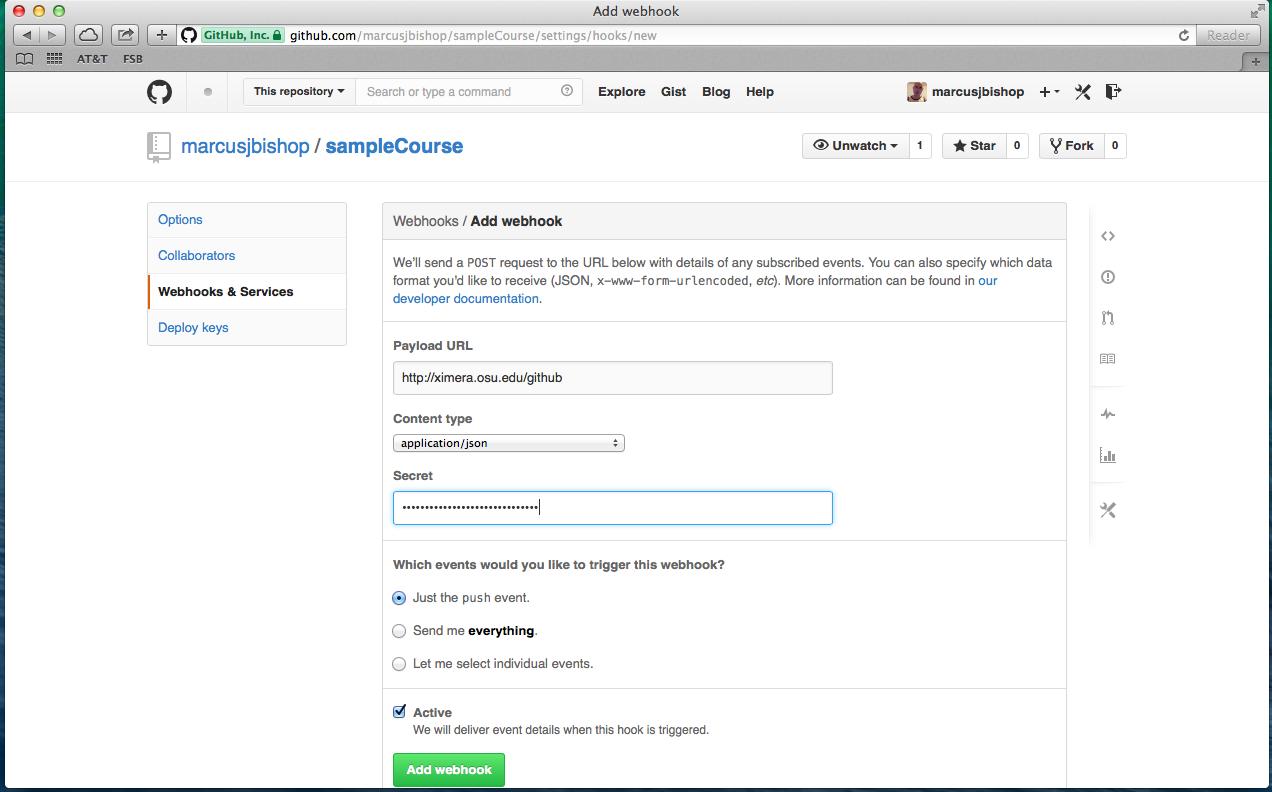
\includegraphics[scale=.3]{Webhook.png}
\end{image}
Finally push the green \verb!Add webhook! button at the bottom.

\item In order to have your course listed on
\href{http://ximera.osu.edu/course}{\tt ximera.osu.edu/course}
you need to \verb!push! the repository.
However, since \verb!git! will not allow a \verb!push!
without any changes to the repository, this is a good point
to add content in the form of a simple exercise.
Update the file \verb!theFirstActivity.tex! 
that you created above so that it looks like the following. 

\begin{verbatim}
\documentclass{ximera}
\title{The First Activity}
\begin{document}
\begin{abstract}
This activity deals with \verb!Ximera! activities.
\end{abstract}
\maketitle
This activity is about creative work.
\begin{exercise}
  Choose the best place to work on mathematics.
  \begin{multipleChoice}
    \choice{At the library}
    \choice[correct]{At the caf\'e}
    \choice{In your office}
  \end{multipleChoice}
\end{exercise}
\end{document}
\end{verbatim}
\begin{remark}
The edits above insert
a multiple-choice question into the \verb!theFirstActivity!
activity. See the Questions and Answers
activity appearing later in this tutorial
for more information on creating exercises.
\end{remark}

\item Change to the top directory \verb!anExampleCourse!
and execute the following commands.
\begin{verbatim}
git commit -am "Added an exercise"
git push
\end{verbatim}
If everything went well, you should find your course listed at 
\href{http://ximera.osu.edu/course}{\tt ximera.osu.edu/course}.
If not, see the troubleshooting activity
or send your questions to
\href{mailto:ximera@math.osu.edu}{\tt ximera@math.osu.edu}.
\begin{remark} The commands above inform \verb!git! that
changes have been made to your repository and 
communicates them to
\href{http://github.com}{\tt github.com}
which in turn communicates them to
\href{http://ximera.osu.edu}{\tt ximera.osu.edu}.
\end{remark}
\end{enumerate}
\end{document}
